% assignment_3.tex
% CS 8735 - Unsupervised Learning (Fall 2015)
%     University of Missouri-Columbia
%             Chanmann Lim
%            October 2015

\documentclass[a4paper]{article}

\usepackage[margin=1 in]{geometry}
\usepackage{listings}
\usepackage{amsmath}
\usepackage{graphicx}
\usepackage{float}
\usepackage{multirow}

\everymath{\displaystyle}
\DeclareMathOperator*{\argmax}{\arg\!\max}
\DeclareMathOperator*{\argmin}{\arg\!\min}

\begin{document}
\setcounter{page}{6}

\noindent The Matlab code for all experiments is in the \textbf{Appendix} section.

\paragraph{6.1.} In this task, we are performing fuzzy c-means clustering with the fuzzifier parameter $q=2$ and distance measure $d(x_i, \theta_j) = (x_i-\theta_j)^TA(x_i-\theta_j)$ with $A=\mathbf{I}$ on GMD dataset from the homework 1 and by considering that there are four significant clusters $m=4$ represented by centroid or mean center.\\

	We randomly initialize the four clusters centroid using uniformly distribution random generator which gives the value between 0 and 1 then we got:

	\begin{align}
		\Theta^{(0)} &= [\theta_1^{(0)} \; \theta_2^{(0)} \; \theta_3^{(0)} \; \theta_4^{(0)}]; \\
			&= \begin{bmatrix}
				0.7802  &  0.6079  &  0.1048  &  0.5495 \\
    			0.3376  &  0.7413  &  0.1279  &  0.4852
			\end{bmatrix}
	\end{align}

	In the fuzzy c-means algorithm, we need to first compute $U = [u_{ij}]$ matrix where

	\begin{align}
		u_{ij} &= u_j(x_i) \\
			&= \frac{1}{\sum_{k=1}^m (\frac{d(x_i,\theta_j)}{d(x_i,\theta_k)})^{\frac{1}{q-1}}}
	\end{align}

	then updating the parameter $\theta_j$ by solving $\sum_{i=1}^N u_{ij}^q \frac{\partial d(x_i,\theta_j)}{\partial \theta_j} = 0$ and we obtain:

	\begin{equation}
		\theta_j = \frac{\sum_{i=1}^N u_{ij}^qx_i}{\sum_{i=1}^N u_{ij}^q}
	\end{equation}

	We repeat this process until the termination criterion $||\Theta(t)-\Theta(t-1)|| < \epsilon$ where $\epsilon = 0.001$ is met and the final values of $\Theta$ (cluster centroids) is:

	\begin{equation}
		\Theta = \begin{bmatrix}
					13.2092  &  0.8970  &  8.5777  &  4.5329 \\
    				2.8618  &  1.7325  &  6.4067  &  6.7135
				\end{bmatrix}
	\end{equation}

\paragraph{6.2.} With the estimated cluster centroids we can perform cluster assignment by assigning each samples to the closest cluster.

\begin{equation}
	k_n^* = \argmin_k ||x_n - \theta_k||^2
\end{equation}

	\begin{figure}[H]
		\centering
			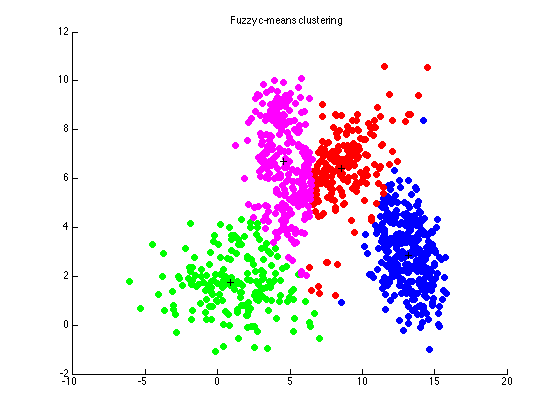
\includegraphics[scale=.55]{images/clusters_plot.png}
		\caption{Plot of samples for different clusters}
	\end{figure}

\paragraph{6.3.} Finally, we computed the total distortion $\sum_{n=1}^N ||x_n-\theta_{k_n}||^2$ for each iteration = [27360, 24016, 17841, 11821, 9014, 7400, 5820, 4925, 4709, 4683, 4689, 4696, 4700, 4704, 4706, 4708, 4709, 4710, 4711, 4712, 4712, 4713, 4713, 4713, 4714, 4714, 4714, 4714, 4714, 4714].

	\begin{figure}[H]
		\centering
			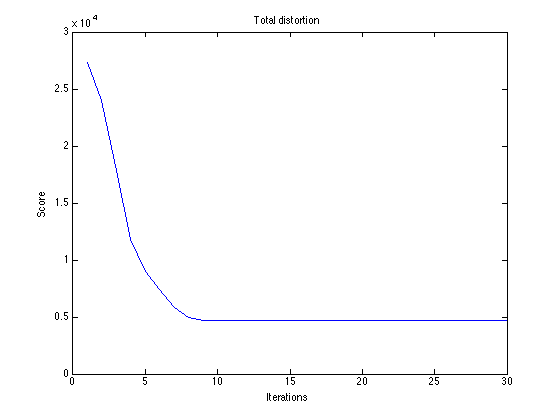
\includegraphics[scale=.55]{images/total_distortion.png}
		\caption{Total distortion}
	\end{figure}
	
\newpage
\subsection*{Appendix:}
	\lstinputlisting[language=Matlab, title=\lstname, basicstyle=\footnotesize]{assignment_3.m}
	\lstinputlisting[language=Matlab, title=\lstname, basicstyle=\footnotesize]{problem_3.m}
	\lstinputlisting[language=Matlab, title=\lstname, basicstyle=\footnotesize]{problem_4.m}
	\lstinputlisting[language=Matlab, title=\lstname, basicstyle=\footnotesize]{linkage.m}
	\lstinputlisting[language=Matlab, title=\lstname, basicstyle=\footnotesize]{vec2cell.m}
	\lstinputlisting[language=Matlab, title=\lstname, basicstyle=\footnotesize]{non_zero_min.m}
	\lstinputlisting[language=Matlab, title=\lstname, basicstyle=\footnotesize]{merge.m}
	\lstinputlisting[language=Matlab, title=\lstname, basicstyle=\footnotesize]{print_cluster.m}
	\lstinputlisting[language=Matlab, title=\lstname, basicstyle=\footnotesize]{fuzzy_c_mean.m}
	\lstinputlisting[language=Matlab, title=\lstname, basicstyle=\footnotesize]{total_distortion.m}
\end{document}